\chapter{Introduksjon}
%--------------------MÅ INN I HOVEDRAPPORT------------------------------------------
\fixme Rotårsaksanalyser er et lite brukt verktøy innen informasjonssikkerhet, men er av økende betydning. Vanlig tilnærming til informasjonssikkerhetsstyring er å utføre en risiko- og sårbarhetsanalyse (ROS-analyse) for så å gjennomføre tiltak som fører risikoene til et akseptabelt nivå. En annen hyppig brukt tilnærming er hendelseshåndtering der en planlegger hvordan det skal responderes på hendelser etter de er inntruffet. Rotårsaksanalyse skiller seg fra disse ved å gå i dybden på problemet, kartlegge hva slags rotårsaker som står bak, og innføre tiltak for å fjerne disse helt.
%%%%%%%%%%%%%%%%%%%%%%%%%%%%%%%%%%%%%%%%%%%%%%%%%%%%%%%%%%%%%%%%%%%%%%%%%%%%%%%%%%%%%

\section{Oppgavebeskrivelse}
Denne rapporten er en delrapport i en større oppgave om rotårsaksanalyse. Dette caset går inn på rotårsaken til at universitetet har så mange kompromitterte brukerkontoer. Når vi snakker om en kompromittert bruker i denne rapporten mener vi at all autentiseringsdata til en brukerkonto er kommet på avveie. I rapporten ser vi på både ansatt- og studentkonto. 

I 2017 var kompromitterte kontoer alene årsaken til omtrent 70 sikkerhetshendelser ved NTNU. I desember 2017 kom det også en stor datadump som innholdt over 5000 kontoer affiliert med NTNU, som alle inneholdt både brukernavn og passord. Av disse var det 101 som fortsatt var aktive i systemene til NTNU, det vil si brukernavn og passord var fortsatt gyldige.

Universitetet kjenner bare årsakene til kompromitteringene i 5 av tilfellene. Phishing sto for fire og spam for en av hendelsene. 

\begin{figure}[H]
    \centering
    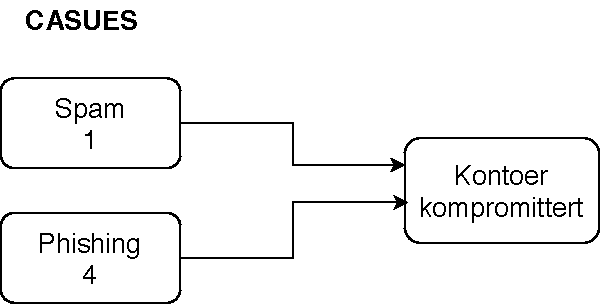
\includegraphics[scale=0.6]{case_2/bilder/kjente_arsaker.pdf}
    \caption[Kjente årsaker til kompromittert konto]{Kjente årsaker til kompromittert konto}
    \label{fig:kjente-arsaker-kompromittert-konto}
\end{figure}

Phishing er en av de få årsakene vi har noe data på, så det er en av årsakene vi vil holde fokus på i analysen. Bildet under viser et eksempel på en phishing e-post som ble sendt til en ansatt ved NTNU.

\begin{figure}[H]%
    \centering
    \subfloat[Forsøk fra November 2017]{{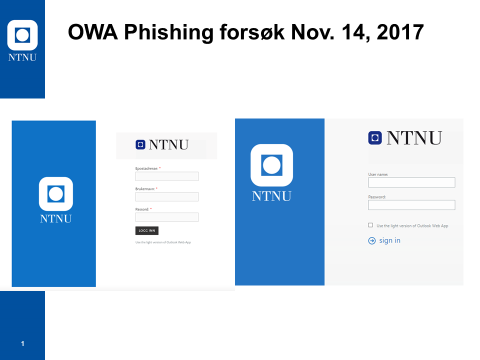
\includegraphics[width=5cm]{case_2/bilder/phishing_1.png} }}%
    \qquad
    \subfloat[Forsøk fra Januar 2018]{{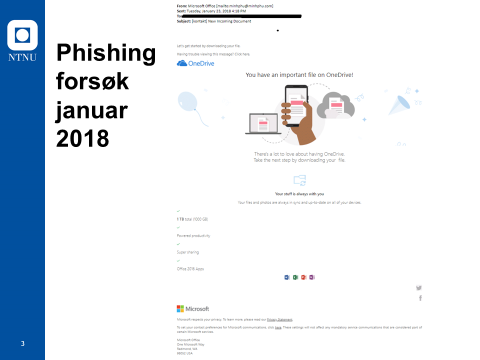
\includegraphics[width=5cm]{case_2/bilder/phishing_2.png} }}%
    \qquad
    \subfloat[Forsøk fra Januar 2018]{{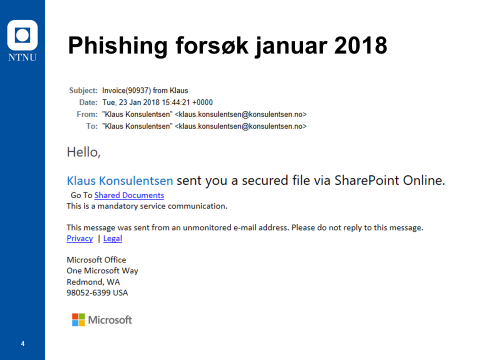
\includegraphics[width=5cm]{case_2/bilder/phishing_3.png} }}%
    \caption{Eksempel på phishing e-post som ble identifisert ved NTNU}%
    \label{fig:example}%
\end{figure}


Universitetet betaler for tilgang til databaser som inneholder tusenvis av forskningsartikler og andre artikler. 26 av de kompromitterte brukerne ble brukt av utenlandske aktører for å skaffe seg tilgang til forskningsartikler. Konsekvensen ved å ha kompromitterte kontoer som laster ned forskningsartikler er ikke bare at NTNU taper penger, men at NTNU risikerer å bli blokkert fra databasene. Angriperne derimot tjener på å ikke trenge å betale for tilgang til databasene. 

Av slike artikler, blir det hentet ut flere tusen på en gang per bruker. Universitetet vet ikke om når det blir hentet ut artikler, eller om det er legitimt bruk av artiklene. De får ofte vite det først når universitetet får beskjed av samarbeidspartnere til NTNU, for eksempel de som tilbyr artiklene. 


Kompromitterte kontoer blir ofte solgt på svartebørsen. 
\begin{figure}[H]
    \centering
    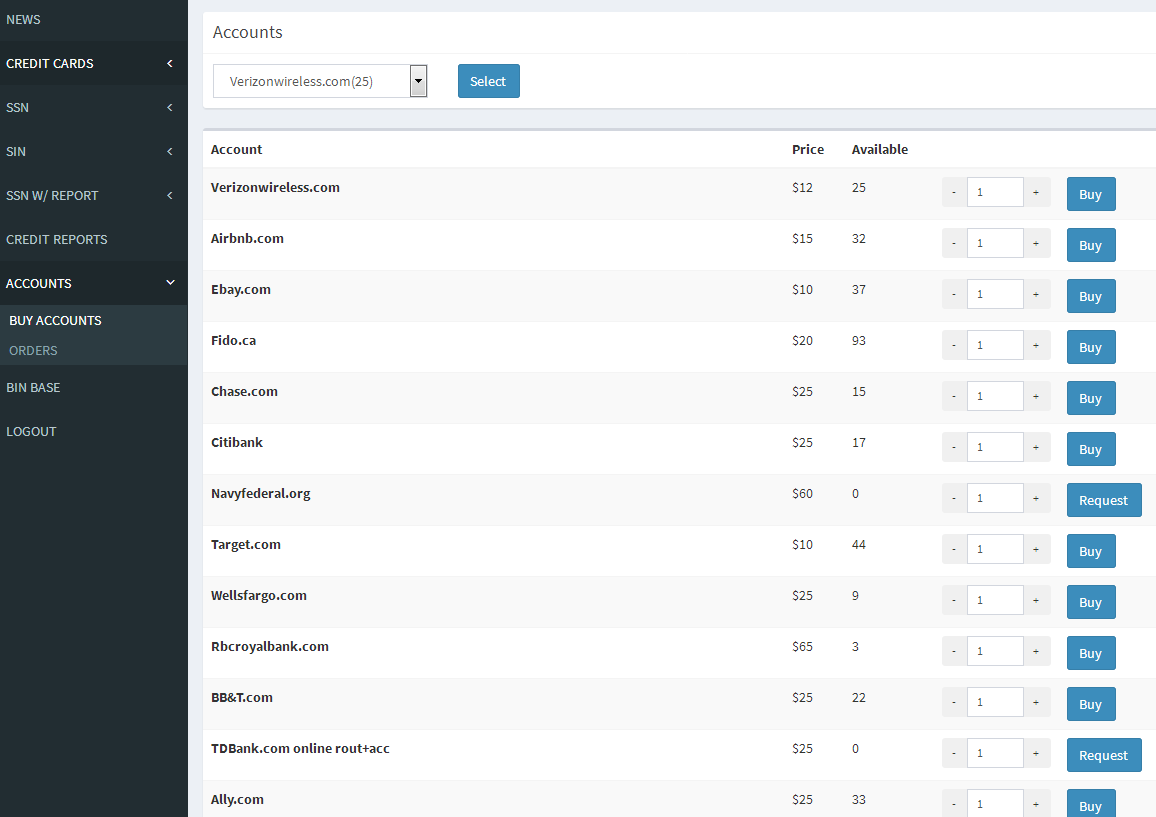
\includegraphics[scale=0.4]{case_2/bilder/prislite_kontore.png}
    \caption[pris-kontoer]{Pris på kontoer}
    \label{fig:pris-kontoer}
\end{figure}
Kilde: https://krebsonsecurity.com/2017/12/the-market-for-stolen-account-credentials/


Dette viser at det er et stort marked for brukerkontoer, og siden NTNU har mange samarbeidspartnere er de et stort mål for trusselaktørene. 


Denne analysen går ut på å identifisere rotårsaken til hvordan NTNU har så mange kompromitterte brukerkontoer, og i løpet av rapporten vil vi svare på følgende forskningsspørsmål:
\begin{itemize}
    \item Hva er rotårsaken til at brukerkontoer ved NTNU blir kompromittert?
    \item Hvordan fungerer rotårsaksanalyse i et case som omhandler misbruk av datakraft?
\end{itemize}


\section{Metode}

Metodebruken i denne analysen er delt inn i syv steg som vist i figur \ref{fig:prosess} under. I hvert steg av denne prosessen brukes det ulike verktøy for å hjelpe til med å forstå problemet, finne rotårsak, og tilslutt implementere tiltak for å eliminere årsakene. Verktøyene fra metoden som blir brukt i hver fase vises til høyre for fasene i figuren under. 
\begin{figure}[H]
    \centering
    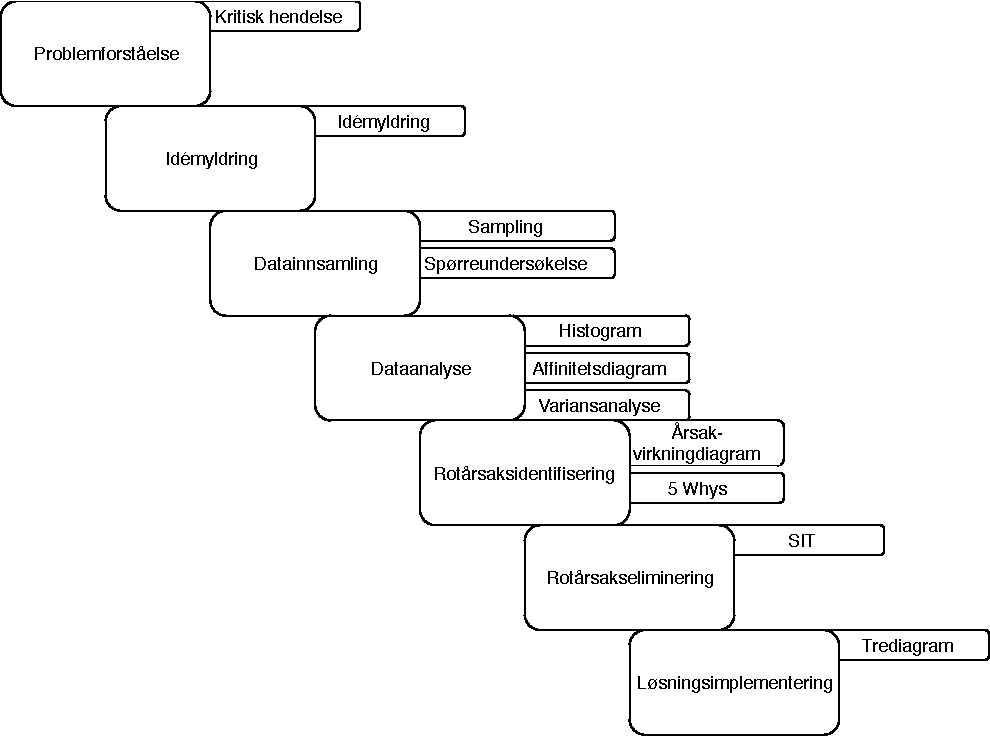
\includegraphics[scale=0.6]{case_2/bilder/RCA-Prosess-case-2.pdf}
    \caption[Rotårsaksanalyseprosessen]{Rotårsaksanalyseprosessen definert av Andersen og Fagerli}
    \label{fig:prosess}
\end{figure}